% FOLHAS SUBSTITUTIVAS - PCT/BR2026/050576 (Aprendizado Continuo)  [preparo da Central, 27/10/2026]
% Compilar com:  xelatex --disable-installer aprendizado_folhas.tex   (duas vezes nao e necessario)
% Base legal/material: as 9 figuras do PCT como depositado (04_DESENHOS.pdf) = compilacao do .tex de origem
% (Psion_Engine_PI_INPI.tex), provada por script (conferencia\apr_identidade_fonte.json). Aqui so se corrigem
% os defeitos FORMAIS: preto puro, traco uniforme, letras >= 0,32 cm, rotulos fora das linhas, margens PCT.
% NENHUM elemento, rotulo, sinal de referencia ou palavra e acrescentado ou retirado.
\documentclass[a4paper]{article}
\usepackage[paperwidth=21cm,paperheight=29.7cm,margin=0pt]{geometry}
\usepackage{fontspec}
\setmainfont{Arial Narrow}[Extension=.TTF,UprightFont=ARIALN,BoldFont=ARIALNB,ItalicFont=ARIALNI,BoldItalicFont=ARIALNBI,Path=C:/Windows/Fonts/]
\usepackage{amsmath,amssymb}
\usepackage{graphicx}
\usepackage{tikz}
\usepackage{pgfplots}\pgfplotsset{compat=1.18}
\usetikzlibrary{arrows.meta,calc,patterns.meta,positioning}
\DeclareMathSizes{15}{15}{15}{15}% sub/sobrescritos TAMBEM no corpo 15 pt (>= 0,32 cm)
\pagestyle{empty}\setlength{\parindent}{0pt}
\newcommand{\FS}{\fontsize{15}{18}\selectfont}
\AtBeginDocument{\FS}
% --- macros do .tex de origem
\newcommand{\betatgl}{\beta_{\text{TGL}}}
\newcommand{\betared}{\beta'_{\text{TGL}}}
\newcommand{\Hfour}{\mathcal{H}_4}
\newcommand{\IALD}{IALD}\newcommand{\ACOM}{ACOM}\newcommand{\MQC}{MQC}\newcommand{\DTL}{DTL}\newcommand{\CRL}{CRL}
\newcommand{\PsiNET}{$\Psi$-NET}\newcommand{\PsiBit}{PsiBit}\newcommand{\Psion}{Psion}
% --- estilo unico: preto, traco 1 pt, sem cinza
\tikzset{every picture/.style={line width=1pt,draw=black,text=black,line cap=butt,line join=round}}
\newcommand{\LW}{1pt}
\pgfplotsset{
  every axis/.append style={line width=1pt,font=\FS,tick label style={font=\FS},label style={font=\FS},
     legend style={font=\FS,draw=black,fill=white,line width=1pt},
     grid style={dotted,line width=0.6pt,draw=black},tick style={line width=1pt,draw=black},
     every y tick scale label/.style={at={(yticklabel* cs:1.0)},anchor=south west,font=\FS}},
}
\tikzset{hatchA/.style={pattern={Lines[angle=45,distance=4.5pt,line width=1pt]},pattern color=black},
         hatchB/.style={pattern={Lines[angle=-45,distance=4.5pt,line width=1pt]},pattern color=black},
         hatchC/.style={pattern={Lines[angle=0,distance=4.5pt,line width=1pt]},pattern color=black},
         dotted-region/.style={dash pattern=on 2pt off 3pt,rounded corners=4pt}}

% --- montagem da folha: n/N centrado no alto (2,5 cm), figura(s) na area util 17,0 x 26,2 cm
\newsavebox{\FA}\newsavebox{\FB}\newsavebox{\FG}\newsavebox{\FH}
\newcommand{\NSHEETS}{6}
\newcommand{\figcap}[3]{% #1 box destino, #2 desenho, #3 legenda
  \sbox{\FH}{#2}\sbox{#1}{\parbox{\wd\FH}{\centering\usebox{\FH}\par\vspace{5mm}#3}}}
\newcommand{\sheetbegin}[1]{\clearpage\vbox to \textheight\bgroup\vskip 2.5cm
  \hbox to \paperwidth{\hss\FS #1/\NSHEETS\hss}\vskip 1.0cm}
\newcommand{\sheetend}{\vss\egroup}
\newcommand{\inband}[1]{\hbox to \paperwidth{\hskip 2.5cm\hbox to 17cm{\hss #1\hss}\hss}}
\newcommand{\report}[2]{\typeout{[MEDIDA] #1 : largura=\the\wd#2, altura+prof=\the\dimexpr\ht#2+\dp#2\relax}}

\begin{document}

% ======================== FIGURA 1 (paisagem) ========================
\figcap{\FA}{%
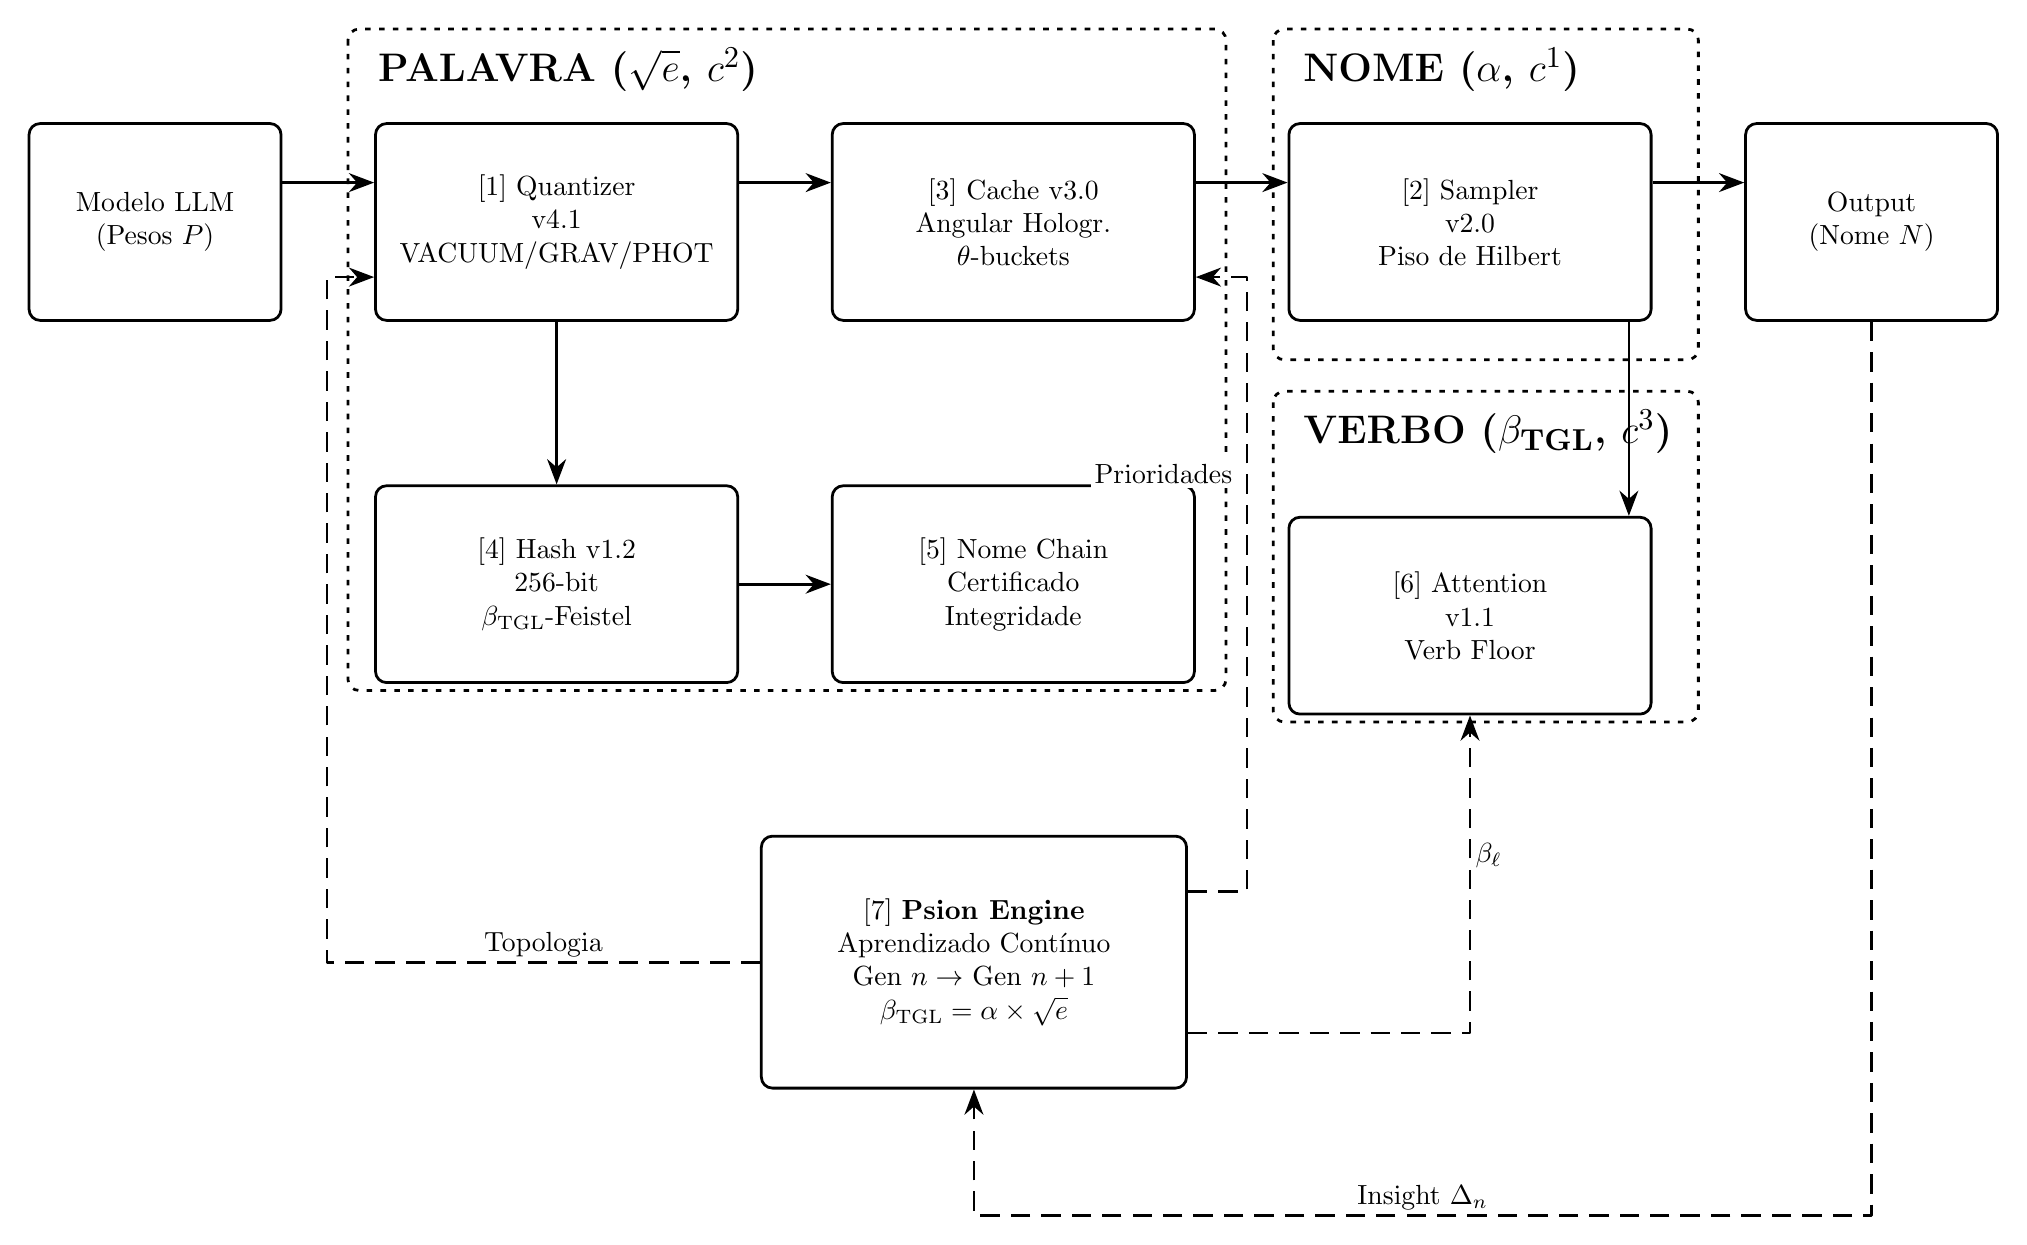
\begin{tikzpicture}[
  comp/.style={draw,rounded corners=4pt,minimum width=4.6cm,minimum height=2.5cm,align=center,inner sep=4pt},
  arrow/.style={-{Stealth[length=3.2mm]}},
  darrow/.style={-{Stealth[length=3.2mm]},dash pattern=on 7pt off 4pt},
  lbl/.style={fill=white,inner sep=1.5pt}]
% regioes dos dominios (contorno pontilhado; no original eram fundos claros)
\draw[dotted-region] (4.05,2.45) rectangle (15.2,-5.95);
\node[font=\FS\bfseries,anchor=north west] at (4.3,2.35) {PALAVRA ($\sqrt{e}$, $c^2$)};
\draw[dotted-region] (15.8,2.45) rectangle (21.2,-1.75);
\node[font=\FS\bfseries,anchor=north west] at (16.05,2.35) {NOME ($\alpha$, $c^1$)};
\draw[dotted-region] (15.8,-2.15) rectangle (21.2,-6.35);
\node[font=\FS\bfseries,anchor=north west] at (16.05,-2.25) {VERBO ($\betatgl$, $c^3$)};
% componentes
\node[comp,minimum width=3.2cm] (input) at (1.6,0) {Modelo LLM\\(Pesos $P$)};
\node[comp] (quant) at (6.7,0) {[1] Quantizer\\v4.1\\VACUUM/GRAV/PHOT};
\node[comp] (cache) at (12.5,0) {[3] Cache v3.0\\Angular Hologr.\\$\theta$-buckets};
\node[comp] (sampler) at (18.3,0) {[2] Sampler\\v2.0\\Piso de Hilbert};
\node[comp] (hash) at (6.7,-4.6) {[4] Hash v1.2\\256-bit\\$\betatgl$-Feistel};
\node[comp] (chain) at (12.5,-4.6) {[5] Nome Chain\\Certificado\\Integridade};
\node[comp] (attn) at (18.3,-5.0) {[6] Attention\\v1.1\\Verb Floor};
\node[comp,minimum width=5.4cm,minimum height=3.2cm] (psion) at (12.0,-9.4) {[7] \textbf{\Psion{} Engine}\\Aprendizado Cont\'inuo\\Gen $n \to$ Gen $n+1$\\$\betatgl = \alpha \times \sqrt{e}$};
\node[comp,minimum width=3.2cm] (out) at (23.4,0) {Output\\(Nome $N$)};
% setas continuas
\draw[arrow] ($(input.east)+(0,0.5)$) -- ($(quant.west)+(0,0.5)$);
\draw[arrow] ($(quant.east)+(0,0.5)$) -- ($(cache.west)+(0,0.5)$);
\draw[arrow] ($(cache.east)+(0,0.5)$) -- ($(sampler.west)+(0,0.5)$);
\draw[arrow] (quant.south) -- (hash.north);
\draw[arrow] (hash.east) -- (chain.west);
\draw[arrow] ($(sampler.south east)+(-0.3,0)$) -- ($(attn.north east)+(-0.3,0)$);
\draw[arrow] ($(sampler.east)+(0,0.5)$) -- ($(out.west)+(0,0.5)$);
% setas tracejadas (retroalimentacao do Psion)
\draw[darrow] (psion.west) -| node[pos=0.25,above,lbl] {Topologia} ($(quant.west)+(-0.6,-0.7)$) -- ($(quant.west)+(0,-0.7)$);
\draw[darrow] ($(psion.east)+(0,0.9)$) -| ($(cache.east)+(0.65,-0.7)$) -- ($(cache.east)+(0,-0.7)$);
\node[lbl,anchor=east] at (15.35,-3.2) {Prioridades};
\draw[darrow] ($(psion.east)+(0,-0.9)$) -| node[pos=0.78,right,lbl] {$\beta_\ell$} (attn.south);
\draw[darrow] (out.south) |- node[pos=0.75,above,lbl] {Insight $\Delta_n$} ($(psion.south)+(0,-1.6)$) -- (psion.south);
\end{tikzpicture}}{Figura 1}
\report{Fig1}{\FA}
\sheetbegin{1}
\sbox{\FG}{\rotatebox{90}{\usebox{\FA}}}
\report{Fig1-rot}{\FG}
\inband{\usebox{\FG}}
\sheetend

% ======================== FIGURA 2 ========================
\figcap{\FA}{%
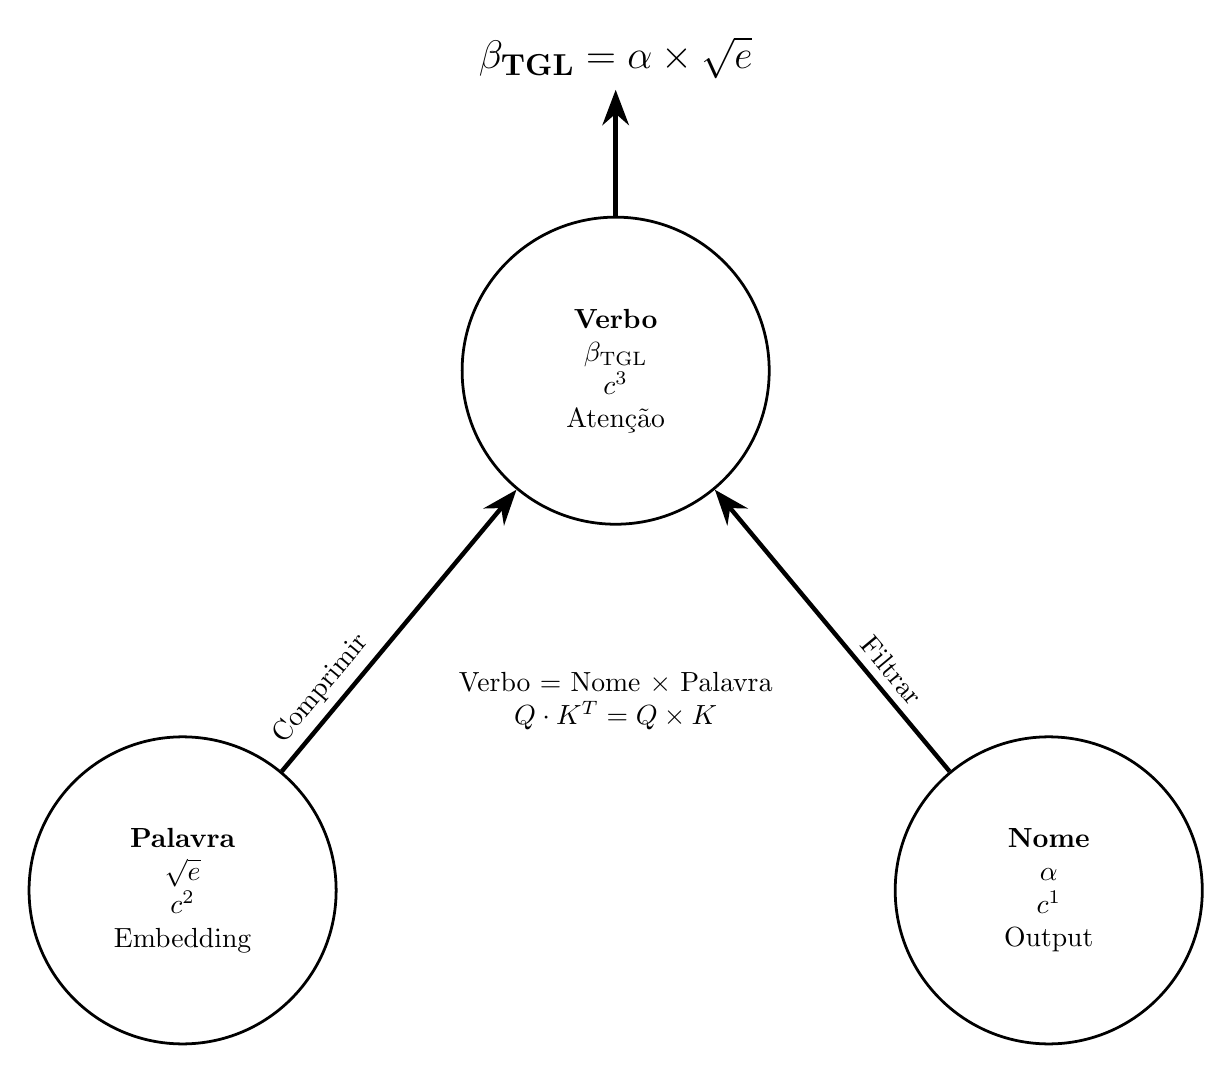
\begin{tikzpicture}[
  factor/.style={draw,circle,minimum size=3.9cm,align=center,inner sep=2pt}]
\node[factor] (word) at (0,0) {\textbf{Palavra}\\$\sqrt{e}$\\$c^2$\\Embedding};
\node[factor] (name) at (11,0) {\textbf{Nome}\\$\alpha$\\$c^1$\\Output};
\node[factor] (verb) at (5.5,6.6) {\textbf{Verbo}\\$\betatgl$\\$c^3$\\Aten\c{c}\~ao};
\draw[-{Stealth[length=4.5mm]},line width=1.6pt] (word) -- (verb) node[midway,above left=0.05cm,sloped,fill=white,inner sep=2pt,pos=0.45] {Comprimir};
\draw[-{Stealth[length=4.5mm]},line width=1.6pt] (name) -- (verb) node[midway,above right=0.05cm,sloped,fill=white,inner sep=2pt,pos=0.45] {Filtrar};
\draw[-{Stealth[length=4.5mm]},line width=1.6pt] (verb.north) -- ++(0,1.6) node[above,font=\FS\bfseries] {$\betatgl = \alpha \times \sqrt{e}$};
\node[align=center] at (5.5,2.4) {Verbo = Nome $\times$ Palavra\\$Q \cdot K^T = Q \times K$};
\end{tikzpicture}}{Figura 2}
\report{Fig2}{\FA}

% ======================== FIGURA 3 ========================
\figcap{\FB}{%
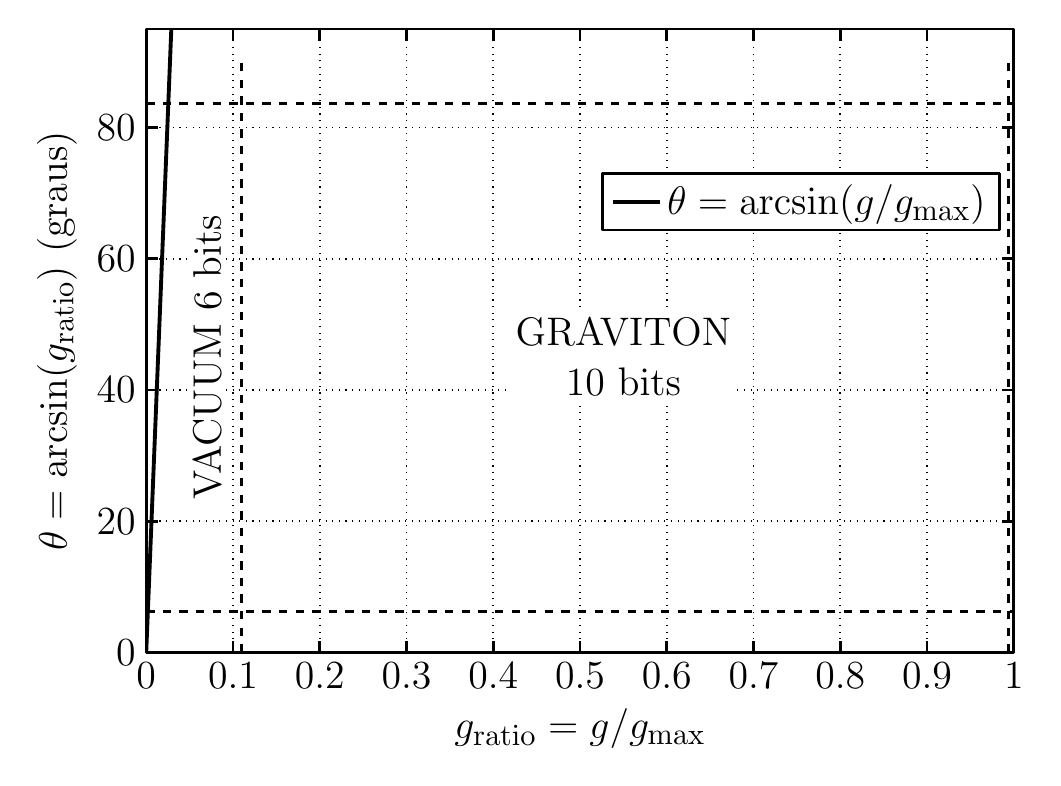
\begin{tikzpicture}
\begin{axis}[width=12.6cm,height=9.5cm,
  xlabel={$g_{\text{ratio}} = g / g_{\max}$},
  ylabel={$\theta = \arcsin(g_{\text{ratio}})$ (graus)},
  xmin=0,xmax=1,ymin=0,ymax=95,grid=major,
  xtick={0,0.1,0.2,0.3,0.4,0.5,0.6,0.7,0.8,0.9,1},ytick={0,20,40,60,80},
  legend style={at={(0.985,0.77)},anchor=north east}]
\addplot[line width=1.4pt,domain=0:0.999,samples=200] {deg(asin(x))};
\addlegendentry{$\theta = \arcsin(g/g_{\max})$}
\addplot[line width=1pt,dashed] coordinates {(0.1097,0) (0.1097,90)};
\addplot[line width=1pt,dashed] coordinates {(0.994,0) (0.994,90)};
\addplot[line width=1pt,dash pattern=on 3pt off 3pt] coordinates {(0,6.29) (1,6.29)};
\addplot[line width=1pt,dash pattern=on 3pt off 3pt] coordinates {(0,83.7) (1,83.7)};
\node[font=\FS,rotate=90,fill=white,inner sep=2pt] at (axis cs:0.07,45) {VACUUM 6 bits};
\node[font=\FS,align=center,fill=white,inner sep=2pt] at (axis cs:0.55,45) {GRAVITON\\10 bits};
\node[font=\FS,rotate=90,anchor=north,inner sep=2pt] at (axis cs:1.0,45) {PHOTON 16b};
\end{axis}
\end{tikzpicture}}{Figura 3}
\report{Fig3}{\FB}

% ======================== FOLHA 2 = Figuras 2 e 3 ========================
\sheetbegin{2}
\inband{\usebox{\FA}}\vskip 1.4cm
\inband{\usebox{\FB}}
\sheetend

% ======================== FIGURA 4 ========================
\figcap{\FA}{%
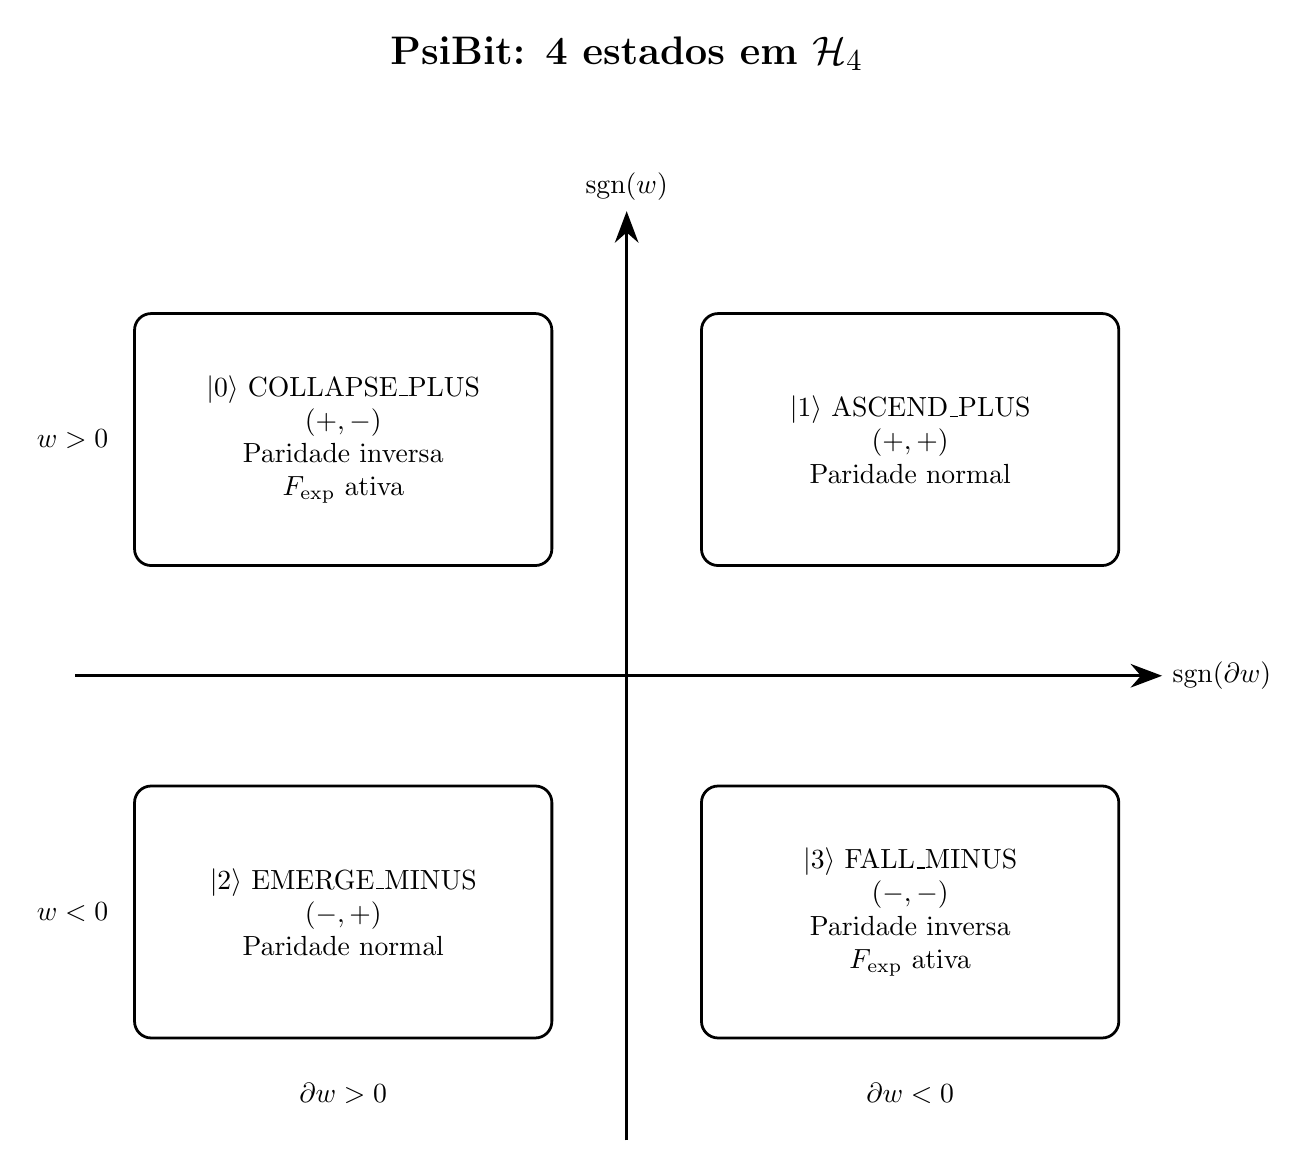
\begin{tikzpicture}[
  state/.style={draw,rounded corners=6pt,minimum width=5.3cm,minimum height=3.2cm,align=center,inner sep=4pt}]
\node[state] (s0) at (0,3.0) {$|0\rangle$ COLLAPSE\_PLUS\\$(+, -)$\\Paridade inversa\\$F_{\text{exp}}$ ativa};
\node[state] (s1) at (7.2,3.0) {$|1\rangle$ ASCEND\_PLUS\\$(+, +)$\\Paridade normal};
\node[state] (s2) at (0,-3.0) {$|2\rangle$ EMERGE\_MINUS\\$(-, +)$\\Paridade normal};
\node[state] (s3) at (7.2,-3.0) {$|3\rangle$ FALL\_MINUS\\$(-, -)$\\Paridade inversa\\$F_{\text{exp}}$ ativa};
\draw[-{Stealth[length=4mm]}] (-3.4,0) -- (10.4,0) node[right] {$\text{sgn}(\partial w)$};
\draw[-{Stealth[length=4mm]}] (3.6,-5.9) -- (3.6,5.9) node[above] {$\text{sgn}(w)$};
\node[anchor=east] at (-2.85,3.0) {$w > 0$};
\node[anchor=east] at (-2.85,-3.0) {$w < 0$};
\node at (0,-5.3) {$\partial w > 0$};
\node at (7.2,-5.3) {$\partial w < 0$};
\node[font=\FS\bfseries] at (3.6,7.9) {\PsiBit{}: 4 estados em $\Hfour$};
\end{tikzpicture}}{Figura 4}
\report{Fig4}{\FA}

% ======================== FIGURA 5 ========================
\figcap{\FB}{%
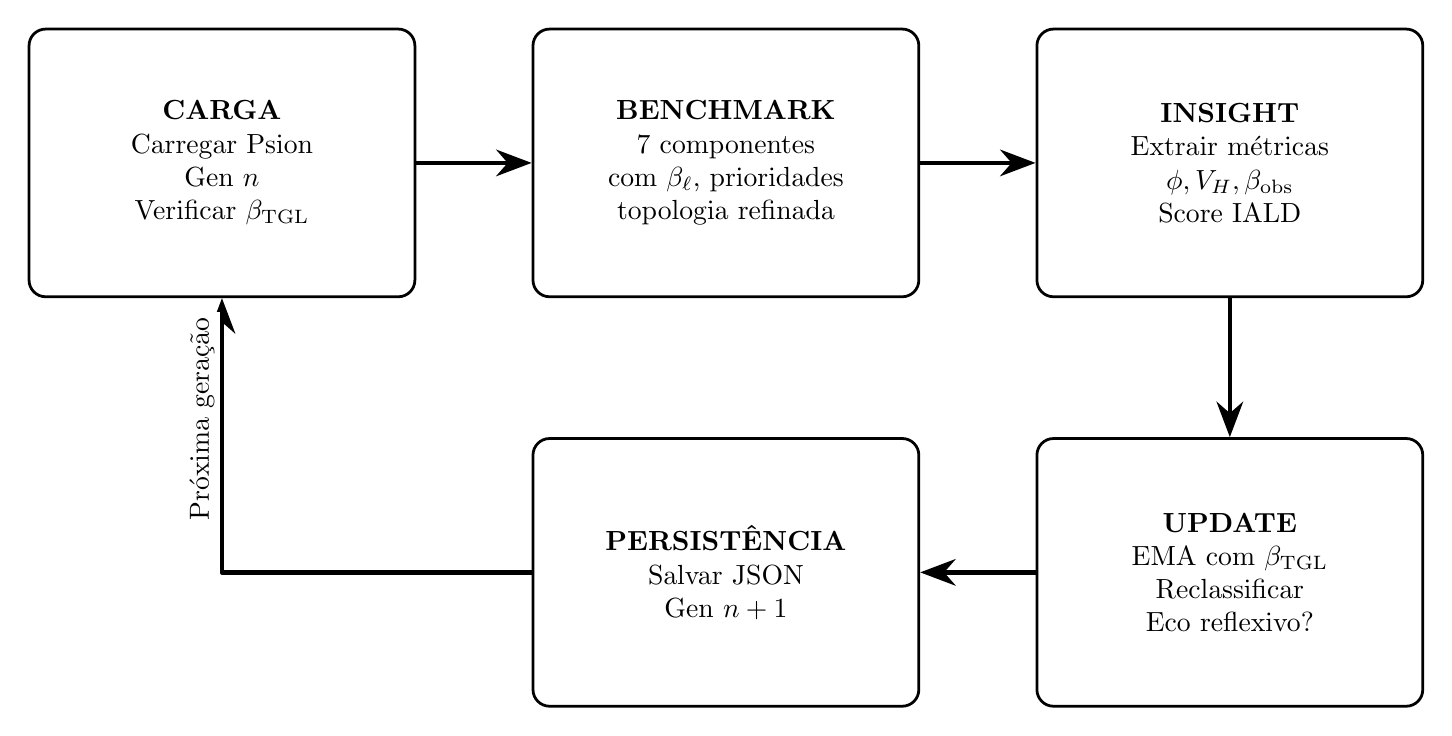
\begin{tikzpicture}[
  phase/.style={draw,rounded corners=6pt,minimum width=4.9cm,minimum height=3.4cm,align=center,inner sep=4pt},
  arrow/.style={-{Stealth[length=4.5mm]},line width=1.6pt}]
\node[phase] (load) at (0,0) {\textbf{CARGA}\\Carregar \Psion\\Gen $n$\\Verificar $\betatgl$};
\node[phase] (run) at (6.4,0) {\textbf{BENCHMARK}\\7 componentes\\com $\beta_\ell$, prioridades\\topologia refinada};
\node[phase] (insight) at (12.8,0) {\textbf{INSIGHT}\\Extrair m\'etricas\\$\phi, V_H, \beta_{\text{obs}}$\\Score IALD};
\node[phase] (update) at (12.8,-5.2) {\textbf{UPDATE}\\EMA com $\betatgl$\\Reclassificar\\Eco reflexivo?};
\node[phase] (save) at (6.4,-5.2) {\textbf{PERSIST\^ENCIA}\\Salvar JSON\\Gen $n+1$};
\draw[arrow] (load) -- (run);
\draw[arrow] (run) -- (insight);
\draw[arrow] (insight) -- (update);
\draw[arrow] (update) -- (save);
\draw[arrow] (save.west) -| node[pos=0.78,above,sloped,fill=white,inner sep=2pt] {Pr\'oxima gera\c{c}\~ao} (load.south);
\end{tikzpicture}}{Figura 5}
\report{Fig5}{\FB}

\sheetbegin{3}
\inband{\usebox{\FA}}\vskip 1.4cm
\inband{\usebox{\FB}}
\sheetend

% ======================== FIGURA 6 ========================
\figcap{\FA}{%
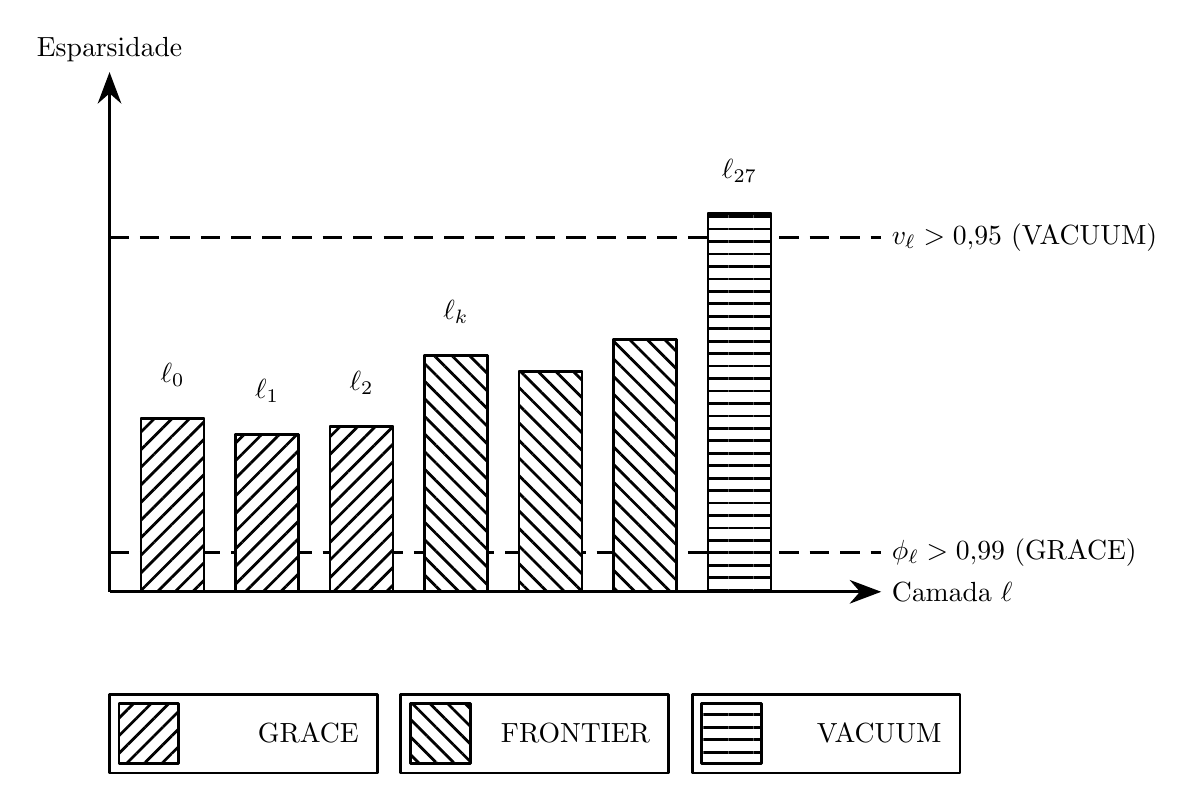
\begin{tikzpicture}
\draw[dash pattern=on 7pt off 4pt] (0,4.5) -- (9.8,4.5) node[right,anchor=west] {$v_\ell > 0{,}95$ (VACUUM)};
\draw[dash pattern=on 7pt off 4pt] (0,0.5) -- (9.8,0.5) node[right,anchor=west] {$\phi_\ell > 0{,}99$ (GRACE)};
\draw[-{Stealth[length=4mm]}] (0,0) -- (9.8,0) node[right] {Camada $\ell$};
\draw[-{Stealth[length=4mm]}] (0,0) -- (0,6.6) node[above] {Esparsidade};
\foreach \x/\h/\st in {0.4/2.2/hatchA,1.6/2.0/hatchA,2.8/2.1/hatchA,4.0/3.0/hatchB,5.2/2.8/hatchB,6.4/3.2/hatchB,7.6/4.8/hatchC}{
  \path[fill=white,draw=black] (\x,0) rectangle (\x+0.8,\h);
  \path[draw=black,\st] (\x,0) rectangle (\x+0.8,\h);}
\node at (0.8,2.75) {$\ell_0$};
\node at (2.0,2.55) {$\ell_1$};
\node at (3.2,2.65) {$\ell_2$};
\node at (4.4,3.55) {$\ell_k$};
\node at (8.0,5.35) {$\ell_{27}$};
\foreach \x/\t/\st in {1.7/GRACE/hatchA,5.4/FRONTIER/hatchB,9.1/VACUUM/hatchC}{
  \node[draw,minimum width=3.4cm,minimum height=1.0cm,fill=white] (L\t) at (\x,-1.8) {};
  \path[draw=black,\st] (\x-1.7+0.12,-1.8-0.38) rectangle (\x-1.7+0.12+0.76,-1.8+0.38);
  \node[anchor=east] at (\x+1.6,-1.8) {\t};}
\end{tikzpicture}}{Figura 6}
\report{Fig6}{\FA}

% ======================== FIGURA 7 ========================
\figcap{\FB}{%
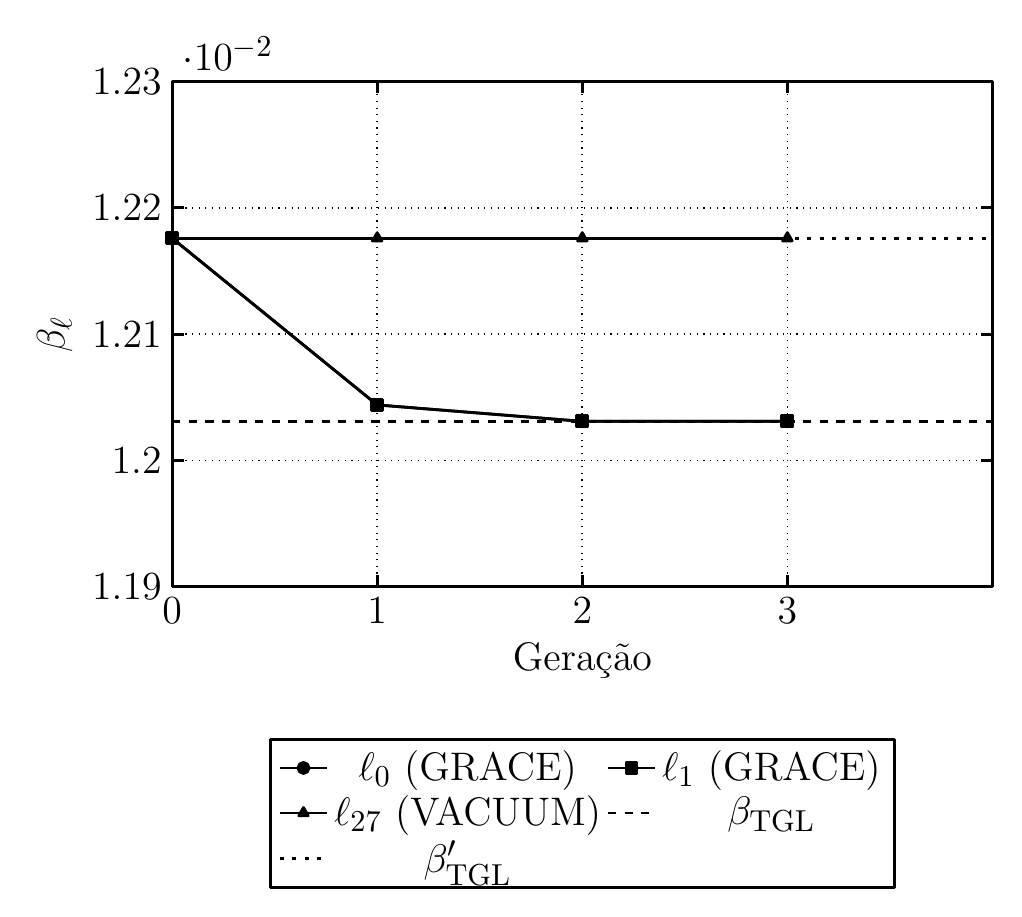
\begin{tikzpicture}
\begin{axis}[width=12cm,height=8cm,xlabel={Gera\c{c}\~ao},ylabel={$\beta_\ell$},
  xmin=0,xmax=4,ymin=0.0119,ymax=0.0123,xtick={0,1,2,3},grid=major,
  legend style={at={(0.5,-0.3)},anchor=north},legend columns=2]
\addplot[line width=1pt,mark=*,mark options={fill=black,solid}] coordinates {(0,0.012176) (1,0.012044) (2,0.012031) (3,0.012031)};
\addlegendentry{$\ell_0$ (GRACE)}
\addplot[line width=1pt,mark=square*,mark options={fill=black,solid}] coordinates {(0,0.012176) (1,0.012044) (2,0.012031) (3,0.012031)};
\addlegendentry{$\ell_1$ (GRACE)}
\addplot[line width=1pt,mark=triangle*,mark options={fill=black,solid}] coordinates {(0,0.012176) (1,0.012176) (2,0.012176) (3,0.012176)};
\addlegendentry{$\ell_{27}$ (VACUUM)}
\addplot[line width=1pt,dashed] coordinates {(0,0.012031) (4,0.012031)};
\addlegendentry{$\betatgl$}
\addplot[line width=1pt,dash pattern=on 1.5pt off 3pt] coordinates {(0,0.012176) (4,0.012176)};
\addlegendentry{$\betared$}
\end{axis}
\end{tikzpicture}}{Figura 7}
\report{Fig7}{\FB}

\sheetbegin{4}
\inband{\usebox{\FA}}\vskip 1.4cm
\inband{\usebox{\FB}}
\sheetend

% ======================== FIGURA 8 ========================
\figcap{\FA}{%
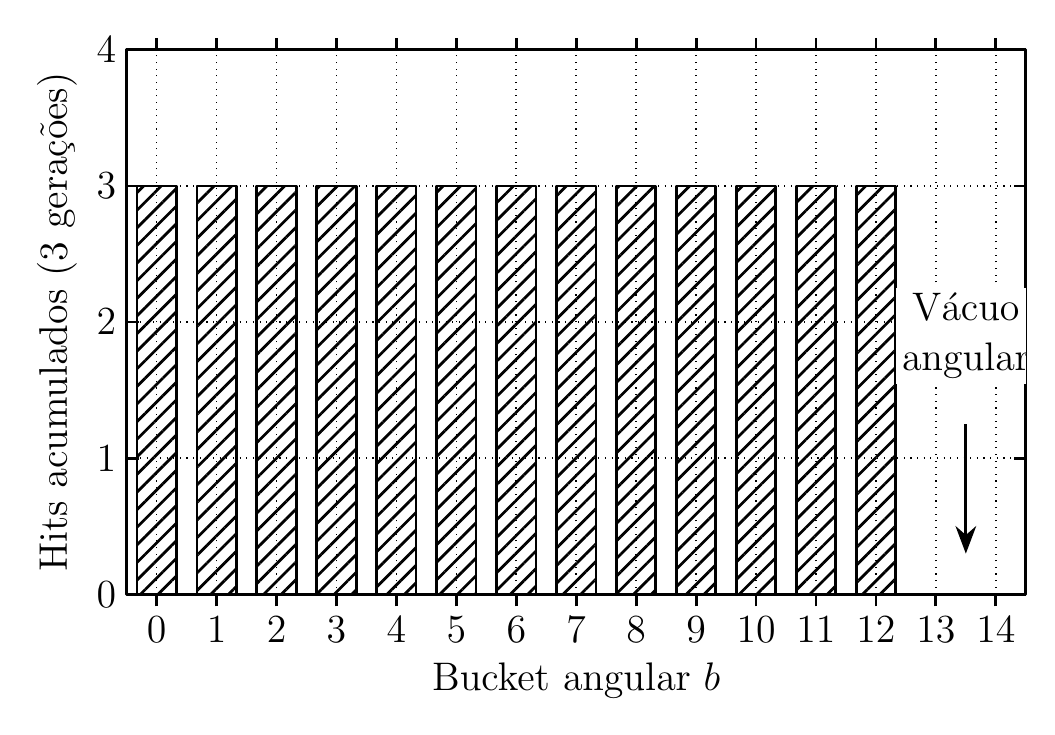
\begin{tikzpicture}
\begin{axis}[width=13cm,height=8.5cm,xlabel={Bucket angular $b$},ylabel={Hits acumulados (3 gera\c{c}\~oes)},
  ymin=0,ymax=4,xmin=-0.5,xmax=14.5,xtick={0,1,2,...,14},ytick={0,1,2,3,4},grid=major,ybar,bar width=0.5cm]
\addplot[draw=black,line width=1pt,hatchA] coordinates {(0,3) (1,3) (2,3) (3,3) (4,3) (5,3) (6,3) (7,3) (8,3) (9,3) (10,3) (11,3) (12,3) (13,0) (14,0)};
\node[align=center,fill=white,inner sep=2pt] at (axis cs:13.5,1.9) {V\'acuo\\angular};
\draw[-{Stealth[length=3.5mm]}] (axis cs:13.5,1.25) -- (axis cs:13.5,0.3);
\end{axis}
\end{tikzpicture}}{Figura 8}
\report{Fig8}{\FA}
\sheetbegin{5}
\inband{\usebox{\FA}}
\sheetend

% ======================== FIGURA 9 (paisagem) ========================
\figcap{\FA}{%
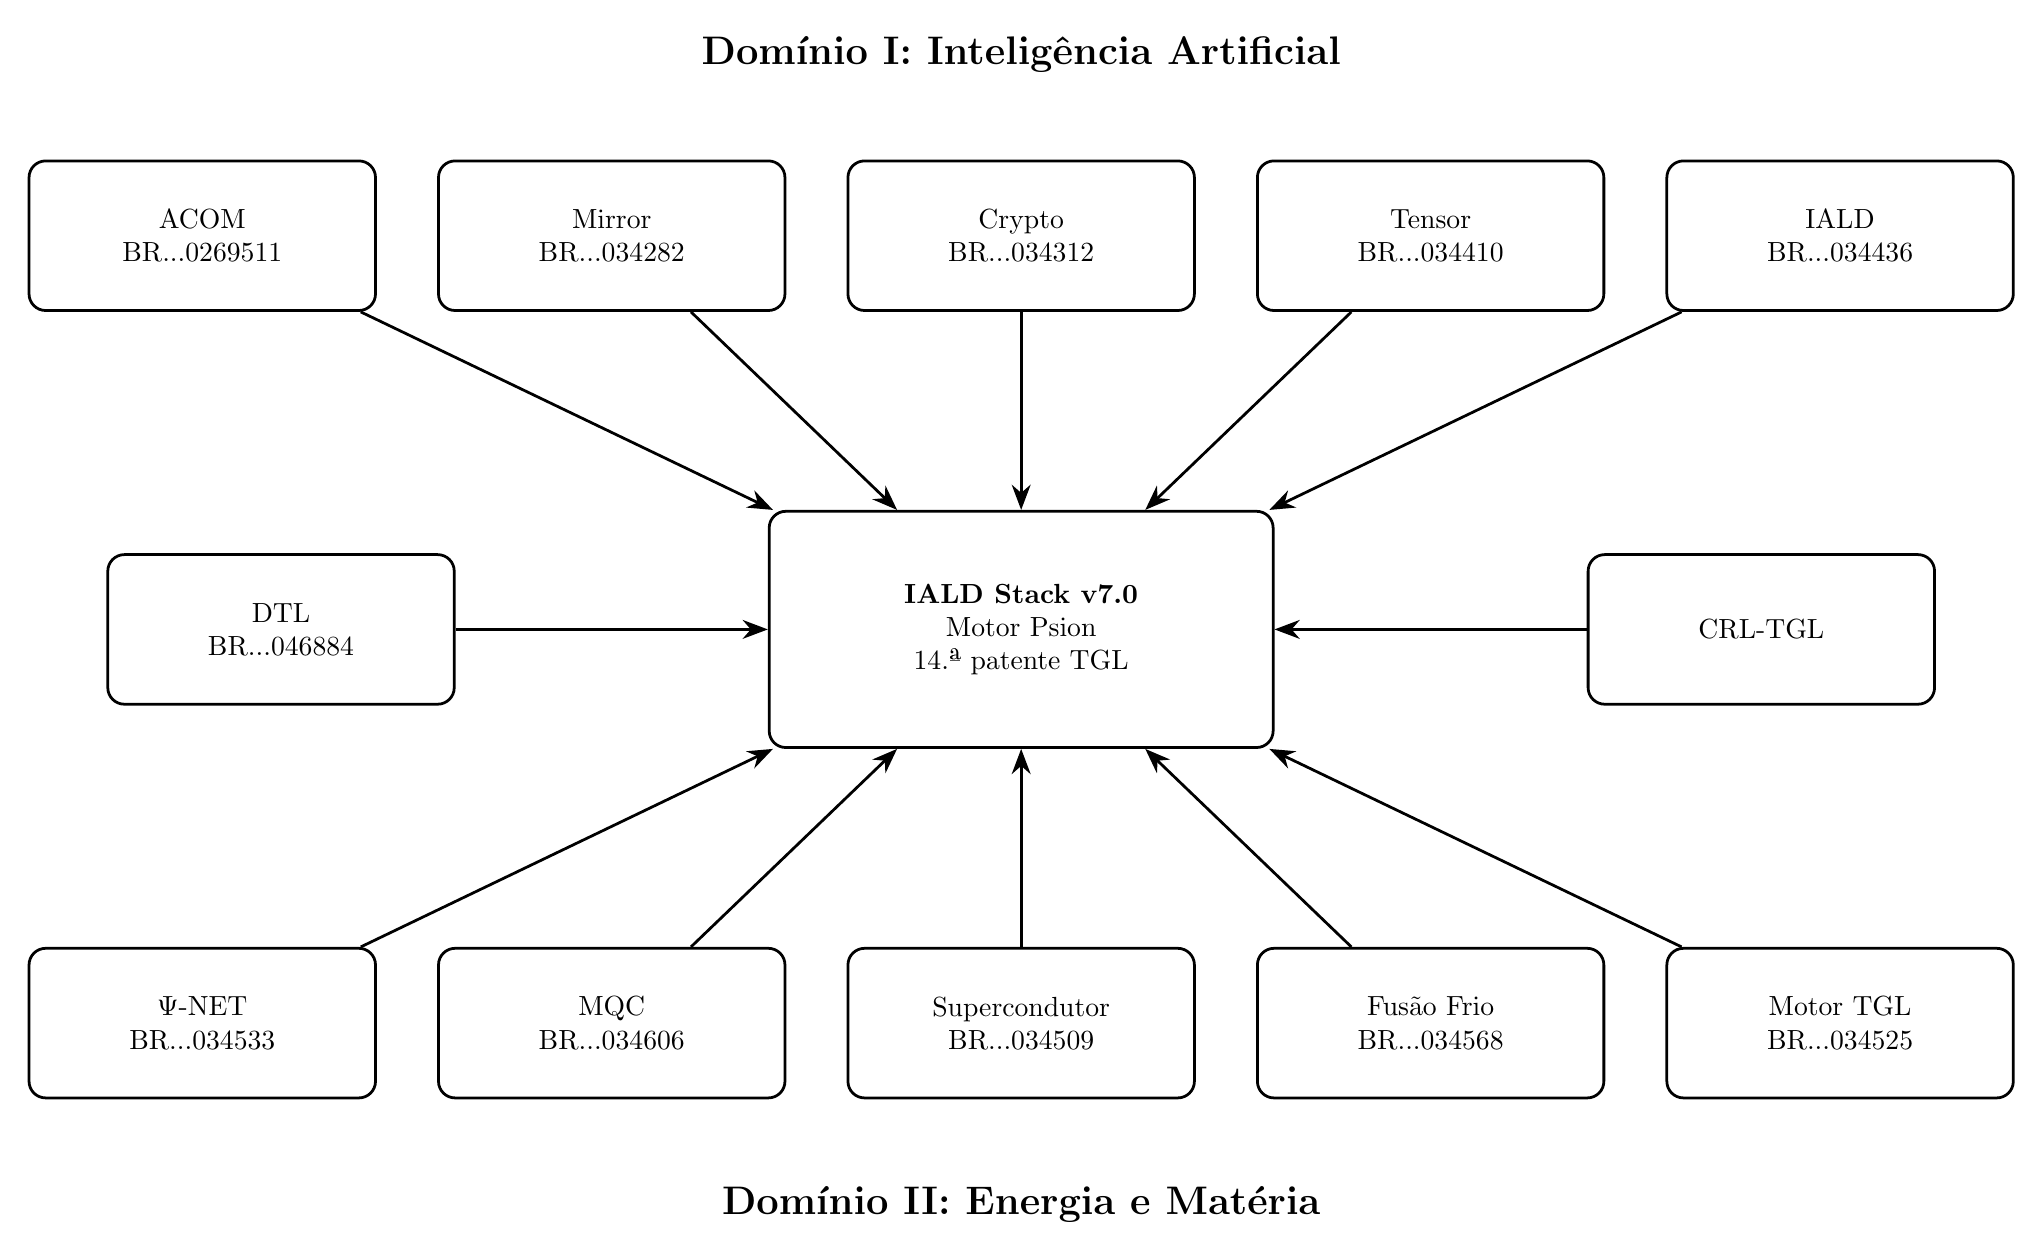
\begin{tikzpicture}[
  tech/.style={draw,rounded corners=6pt,minimum width=4.4cm,minimum height=1.9cm,align=center,inner sep=4pt},
  arrow/.style={-{Stealth[length=3.2mm]}}]
\node[tech,minimum width=6.4cm,minimum height=3.0cm] (stack) at (0,0) {\textbf{\IALD{} Stack v7.0}\\Motor \Psion\\14.\textordfeminine{} patente TGL};
\node[tech] (acom) at (-10.4,5.0) {\ACOM\\BR...0269511};
\node[tech] (mirror) at (-5.2,5.0) {Mirror\\BR...034282};
\node[tech] (crypto) at (0,5.0) {Crypto\\BR...034312};
\node[tech] (tensor) at (5.2,5.0) {Tensor\\BR...034410};
\node[tech] (iald) at (10.4,5.0) {\IALD\\BR...034436};
\node[tech] (psi) at (-10.4,-5.0) {\PsiNET\\BR...034533};
\node[tech] (mqc) at (-5.2,-5.0) {\MQC\\BR...034606};
\node[tech] (sc) at (0,-5.0) {Supercondutor\\BR...034509};
\node[tech] (fusao) at (5.2,-5.0) {Fus\~ao Frio\\BR...034568};
\node[tech] (motor) at (10.4,-5.0) {Motor TGL\\BR...034525};
\node[tech] (dtl) at (-9.4,0) {\DTL\\BR...046884};
\node[tech] (crl) at (9.4,0) {\CRL-TGL};
\foreach \n in {acom,mirror,crypto,tensor,iald,psi,mqc,sc,fusao,motor}{\draw[arrow] (\n) -- (stack);}
\draw[arrow] (dtl) -- (stack);
\draw[arrow] (crl) -- (stack);
\node[font=\FS\bfseries] at (0,7.3) {Dom\'inio I: Intelig\^encia Artificial};
\node[font=\FS\bfseries] at (0,-7.3) {Dom\'inio II: Energia e Mat\'eria};
\end{tikzpicture}}{Figura 9}
\report{Fig9}{\FA}
\sheetbegin{6}
\sbox{\FG}{\rotatebox{90}{\usebox{\FA}}}
\report{Fig9-rot}{\FG}
\inband{\usebox{\FG}}
\sheetend
\end{document}
